\documentclass[12pt,a4paper,openright,twoside]{book}
\usepackage[utf8]{inputenc}
\usepackage{disi-thesis}
\usepackage{code-lstlistings}
\usepackage{notes}
\usepackage{shortcuts}
\usepackage{acronym}

\school{\unibo}
\programme{Corso di Laurea Triennale in Ingegneria e Scienze Informatiche}
\title{Open Source Face Image Quality: valutazione e contribuzione}
\author{Senni Mattia}
\date{\today}
\subject{Visione Artificiale}
\supervisor{Franco Annalisa}
\cosupervisor{Borghi Guido}
\session{II}
\academicyear{2024-2025}

% Definition of acronyms
\acrodef{IoT}{Internet of Thing}
\acrodef{vm}[VM]{Virtual Machine}


\mainlinespacing{1.241} % line spacing in mainmatter, comment to default (1)

\begin{document}

\frontmatter\frontispiece

\begin{abstract}	
La visione artificiale sta venendo sempre più utilizzata nel riconoscimento di un soggetto tramite immagini facciali, ambito in cui si stanno diffondendo sistemi di riconoscimento biometrico automatico.
In questi contesti, è fondamentale garantire un'acquisizione controllata e standardizzata delle immagini facciali, al fine di ridurre errori di riconoscimento e vulnerabilità a minacce come il face morphing.
Una cattiva acquisizione può compromettere l’intero processo biometrico, rendendo il sistema suscettibile a falsificazioni e riducendone l’affidabilità.
Questo progetto contribuisce allo sviluppo ed alla valutazione di un software che ha l'obbiettivo di implementare un draft ISO, volto a valutare la qualità dell'acquisizione delle immagini facciali secondo diverse metriche.
\end{abstract}

% \begin{dedication} % this is optional
% Optional. Max a few lines.
% \end{dedication}

%----------------------------------------------------------------------------------------
\tableofcontents   
\listoffigures     % (optional) comment if empty
\lstlistoflistings % (optional) comment if empty
%----------------------------------------------------------------------------------------

\mainmatter

%----------------------------------------------------------------------------------------
\chapter{Introduzione}
\label{chap:introduzione}
%----------------------------------------------------------------------------------------
\section{Motivazioni}
Nell’ambito della visione artificiale, e in particolare del riconoscimento facciale, si è ottenuta negli ultimi anni a una significativa riduzione dei tassi di errore grazie all’introduzione di algoritmi basati su tecniche di deep learning.
Tuttavia, gli errori di riconoscimento rimangono ancora rilevanti e possono essere influenzati da numerosi fattori, tra cui le modalità di acquisizione dell’immagine, la cooperazione del soggetto durante la cattura biometrica, la specifica implementazione dell’algoritmo di confronto e la logica decisionale associata.
In questo contesto, risulta evidente la necessità di un ammodernamento sostanziale delle procedure di acquisizione, per evitare un peggioramento delle prestazioni dei sistemi biometrici a fronte dell’incremento dei volumi di dati da elaborare.
L’urgenza di intervenire su questi aspetti si collega anche a una maggiore consapevolezza dell’importanza dell’usabilità dei sistemi biometrici, sia per gli utenti finali sia per gli operatori umani, i quali possono contribuire in modo significativo alla riduzione degli errori attraverso una migliore qualità nella fase di acquisizione.
Spesso, infatti, un sistema progettato esclusivamente sulla base della tecnologia rischia di mostrare i propri limiti se non considera in modo integrato le dinamiche dell’interazione umana.
Parallelamente, l’adozione crescente del riconoscimento facciale in contesti di ampia scala, come la gestione dell’identità civile, le applicazioni commerciali e le attività di controllo delle forze dell’ordine, ha comportato la raccolta massiva di immagini del volto, che fungono sia da campioni di riferimento in fase di registrazione sia da elementi di confronto successivo.
Programmi di portata nazionale e internazionale, come quelli attivati in Cina, nell’Unione Europea, negli Stati Uniti e in India, testimoniano il crescente impiego di questa tecnologia in settori critici quali i trasporti, l’immigrazione e l’autenticazione dell’identità.
Tuttavia, molte delle immagini facciali oggi raccolte provengono da dispositivi di acquisizione non specificamente progettati per l'acquisizione di immagini del volto.
Le immagini destinate a documenti d’identità o a database ufficiali vengono per lo più acquisite con telecamere configurate secondo specifiche documentarie, come lo standard ISO/IEC 39794-5, che disciplina l’inquadratura e le caratteristiche fotografiche.
In assenza di strumenti automatici di valutazione della qualità, la conformità viene spesso affidata al fotografo.
A questo si aggiunge il problema rappresentato da comportamenti involontari dei soggetti durante la cattura, portando ad una  variazioni tra l’immagine di riferimento e quella di confronto, compromettendo l’efficacia del riconoscimento.
È pertanto essenziale garantire la coerenza con la presentazione canonica prevista dagli standard, ossia un volto centrato e frontale, con espressione neutra, occhi aperti e privo di occhiali.
Considerando la grande eterogeneità degli utenti, per età, costituzione fisica, etnia, lingua, cultura, alfabetizzazione e familiarità con la tecnologia, è evidente l'importanza di un’attenta progettazione dal punto di vista dei fattori umani per migliorare l'acquisizione delle immagini facciali.
Un’ulteriore criticità risiede nella separazione tra il processo di acquisizione dell’immagine e quello di valutazione della qualità, che spesso avviene solo in un secondo momento, quando la fotografia viene inviata a un server remoto.
Se la qualità dell’immagine risulta inadeguata, si rende necessaria una nuova acquisizione aggravando tempi e costi.
In questo scenario, il lavoro descritto da questa tesi si colloca nell’ambito della contribuzione e valutazione di un software conforme al draft della normativa ISO 29794-5:2024, la quale stabilisce requisiti specifici del  software implementante l’analisi di una singola immagine facciale.
\section{Obbiettivo}
Il progetto consiste in una valutazione del software OFIQ (Open Source Face Image Quality), strumento open source sviluppato per implementare le metriche descritte nel draft dello standard ISO precedentemente illustrato. Il lavoro consiste inoltre nella contribuzione allo sviluppo del software mediante l’implementazione di ulteriori metriche previste o suggerite dallo standard, ma non ancora integrate nel software. L’obiettivo principale è quello di verificare l’affidabilità di OFIQ per il controllo di qualità delle immagini facciali destinate all’identificazione biometrica, testandolo su esempi conformi alle specifiche e su esempi non conformi. Si vuole valutare se l’impiego del software durante la fase di acquisizione possa rappresentare uno strumento accurato per garantire la qualità e la conformità delle immagini biometriche.  

\section{Metodo}
Per la realizzazione di questo progetto si è partiti con la comprensione delle varie metriche descritte nel draft ISO 29794-5:2024.
Successivamente si è testata ogni singola metrica comparando diversi dataset divisi tra immagini che soddisfano i requisiti dello standard e immagini che non soddisfano la determinata metrica che si sta valutando, in seguito a queste valutazioni si guarda la distribuzioni 

\paragraph{Structure of the Thesis}

\note{At the end, describe the structure of the paper}

\chapter{State of the art}

I suggest referencing stuff as follows: \cref{fig:random-image} or \Cref{fig:random-image}

\begin{figure}
    \centering
    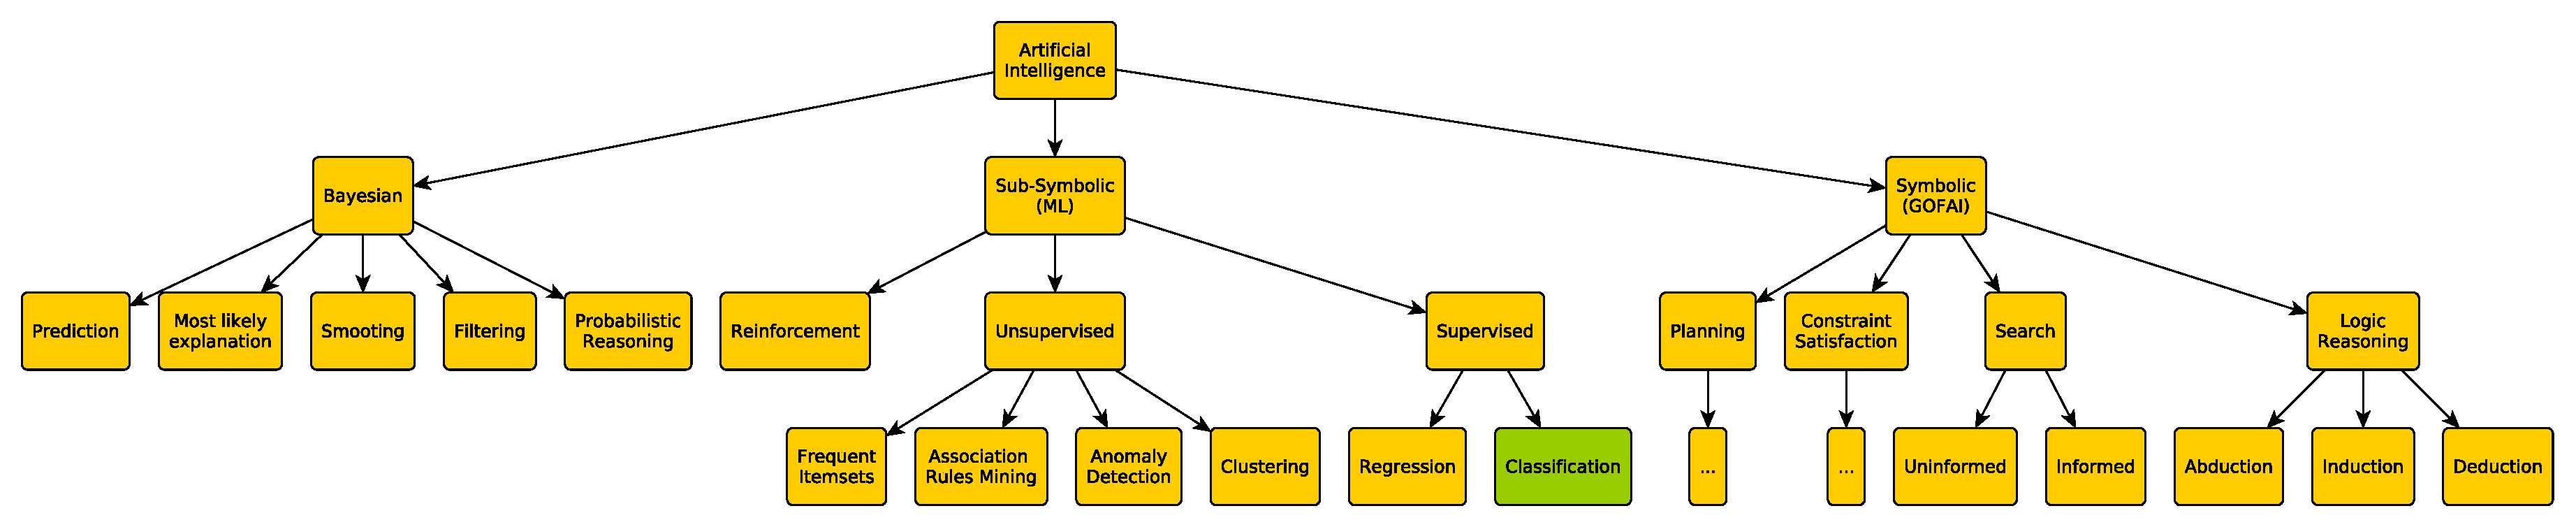
\includegraphics[width=.8\linewidth]{figures/random-image.pdf}
    \caption{Some random image}
    \label{fig:random-image}
\end{figure}

\section{Some cool topic}

\chapter{Contribution}

You may also put some code snippet (which is NOT float by default), eg: \cref{lst:random-code}.

\lstinputlisting[float,language=Java,label={lst:random-code}]{listings/HelloWorld.java}

\section{Fancy formulas here}

%----------------------------------------------------------------------------------------
% BIBLIOGRAPHY
%----------------------------------------------------------------------------------------

\backmatter

\nocite{*} % Remove this as soon as you have the first citation

\bibliographystyle{alpha}
\bibliography{bibliography}

\begin{acknowledgements} % this is optional
Optional. Max 1 page.
\end{acknowledgements}

\end{document}
